% !TEX encoding = UTF-8
% !TEX program = pdflatex
% !TEX root = InformationRetrieval.tex
% !TEX spellcheck = it-IT

% 10 Novembre 2016
%\section{Modello probabilistico}
%\subsection{Basi di probabilità}
%\subsubsection{Interpretazione grafica del costo degli errori}

\chapter{Sistemi di reperimento dell'informazione}

In questa parte parleremo dei sistemi di reperimento che sono disponibili su internet e che sono pronti all'uso.

\section{Sistemi open-source}

I 3 principali sistemi di IR disponibili sul mercato open-source sono:

\begin{itemize}
	\item \textbf{Apache Lucene}: viene tipicamente utilizzato all'interno di \textbf{Apache Solr}, una soluzione che permette di creare dei motori di ricerca ad-hoc per l'ambito enterprise.
	\item \textbf{Terrier}: progetto accademico che raramente viene utilizzato a livello commerciale.
	\item \textbf{Indri}: sistema orientato verso modelli di reperimento che utilizzano language modelling (cose avanzate che probabilmente non affronteremo).
\end{itemize}

\noindent Tutti questi sistemi permettono di:

\begin{itemize}
	\item Indicizzare collezioni di documenti, con analisi lessicale, stop-list, stemmer e creazione di indice.
	\item Indicizzare ed elaborare le query.
	\item Reperire documenti producendo delle liste ordinate in base alla rilevanza (ranking).
	\item Utilizzare diversi modelli di reperimento: booelano, vettoriale, probabilistico.
\end{itemize}

\noindent Tutti questi sistemi sono pensati per gestire la lingua inglese, ma permettono comunque di utilizzare altre lingue.


\subsection{Apache Lucene}

Sistema open-source dell'Apache Software Foundation, creato del 1999, tipicamente utilizzato all'interno di sistemi commerciali.

\subsection{Terrier}

Sviluppato dal gruppo di ricerca dell'Università di Glasgow a partire dal 2001.

L'implementazione del sistema è quello che è, perché viene sviluppato a pezzi da vari studenti/ricercatori.

L'utilizzo tipico di questo sistema è in ambito accademico o nel mondo della ricerca.

Prevede dei modelli di \textit{learning to rank}, ovvero modelli che apprendono come fare ranking guardando come altri modelli hanno fatto ranking per la stessa query. 

\subsection{Indri}

Sempre sviluppato da un'università, scritto in C++ e tipicamente utilizzato in ambiti di ricerca.

Viene utilizzata con la libreria RankLib e  implementa vari algoritmi di \textit{learning to rank}.

\section{Funzionamento di Terrier}

Per utilizzarlo è necessario scaricare l'installer dal sito \url{http://www.terrier.org}.

Dopo l'installazione, che alla fine è la decompressione di un pacchetto, vengono create un po' di cartelle. Quelle più interessanti sono:

\begin{itemize}
	\item \texttt{bin}: contiene gli script e i file eseguibili.
	\item \texttt{etc}: contiene i file di configurazione \texttt{terrier.properties} e \texttt{collection.spec}
	\item \texttt{target/lib}: contiene i file jar, tra cui quelli di Terrier. Qui va messa la nostra versione di Terrier modificata.
	\item \texttt{var}: contiene l'indice e i file dei risultati.
\end{itemize}


\subsection{Properties}

Il file con tutta la configurazione di sistema si trova su \texttt{etc/terrier}.
IN questo file è possibile specificare quali file indicizzare, quale tokenizer utilizzare, stop-list, stemmer, ecc.

\todo{Nel progetto conviene utilizzare un file properties simile.}

\subsection{Documentazione}

Nel sito web si trova la documentazione completa del sistema, non solo la JavaDoc, ma anche la descrizione del funzionamento di Terrier, con anche degli esempi di utilizzo.

\section{Indicizzazione con Terrier}

\begin{figure}[htbp]
	\centering
	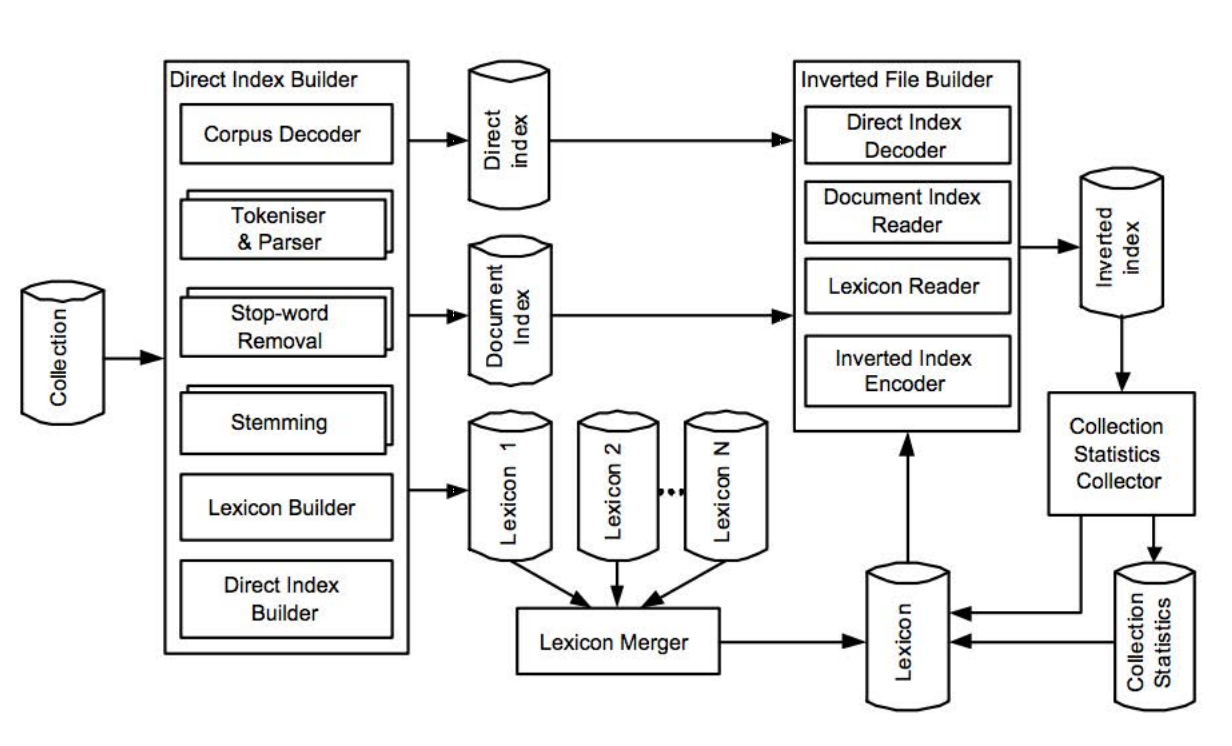
\includegraphics[width=0.9\linewidth]{images/l12-fig-1.png}
\end{figure}

Si parte da una collezione di documenti (corpus), sulla quale viene costruito l'indice diretto, con le fasi viste precedentemente.
La costruzione del lexicon (dizionario) viene fatta prima costruendo \textit{N} dizionari per i vari documenti, che poi vengono uniti in modo automatico. Il dizionario generato contiene delle statistiche relative al \textit{tf} e \textit{idf}.

Viene poi creato l'indice inverso che contiene un po' di informazioni relative ai termini. Tipicamente è presente tutto quello che serve, ma può capitare che sia necessario modificare la creazione dell'indice per avere a disposizione informazioni extra, utili ai modelli di reperimento.

\subsection{Un esempio di indicizzazione}

Supponiamo di voler indicizzare i file presenti all'url \url{http://www.dei.unipd.it/~silvello/IR2016-2017/small_test_collections/text/} e che siano presenti in locale nel percorso \texttt{ /IR2016-2017/collections/text/}.

Il primo passo è andare a specificare all'interno del file \texttt{etc/collection.spec} quali file indicizzare, indicandone il percorso assoluto.
Si può fare a mano, oppure si può fare in modo automatico utilizzando uno script bash:

\begin{center}
	\texttt{sh bin/trec\_setup.sh /path-to-collection/}
\end{center}

\noindent Serve poi ri-configurare il file di properties, perché ad ogni esecuzione di \texttt{trec\_steup} viene inizializzato.

\begin{figure}[htbp]
	\centering
	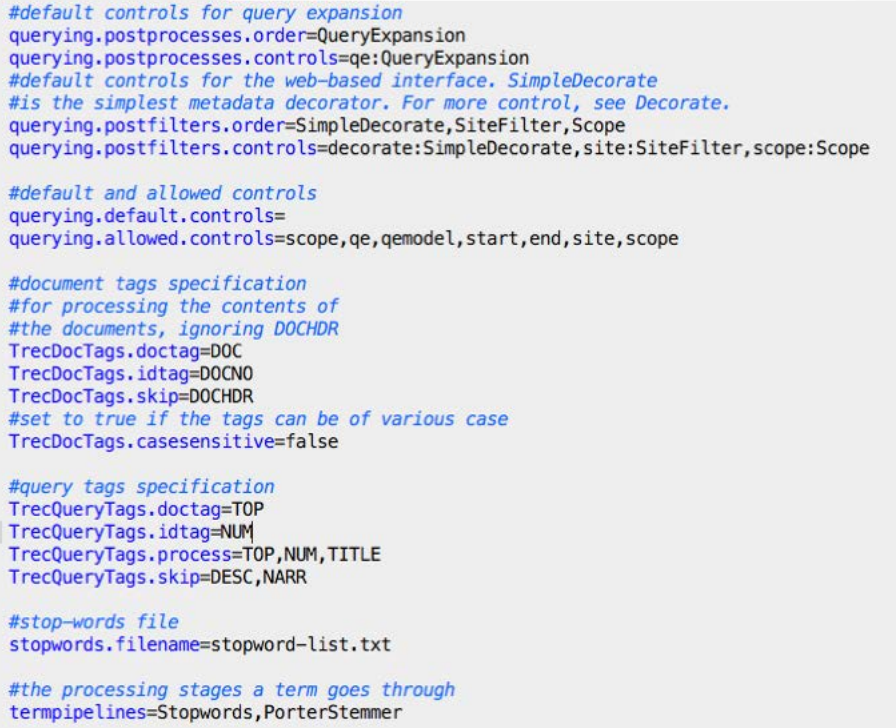
\includegraphics[width=0.8\linewidth]{images/l12-fig-2.png}
\end{figure}

\noindent Il primo blocco (1-11) riguarda le funzionalità di query expansion e la possibilità di utilizzare Terrier come applicazione web. A noi questa cosa non ci interessa.

Il secondo blocco (13-26) riguarda le proprietà per la valutazione sperimentale di un sistema IR. Servono per specificare quali tag devono essere indicizzati\footnote{Nel caso di documenti strutturati}. Il tutto sarà più chiaro dopo aver fatto la parte di valutazione.

Il terzo blocco (28-32) contiene il percorso per raggiungere il file contenente le stop-word e la configurazione della pipeline di indicizzazione dei termini.
Per usare il nostro stemmer dovremmo specificare un \texttt{LookupStemmer}, mentre per ottenere l'indice puro dei termini è necessario lasciare il campo vuoto.

\begin{figure}[htbp]
	\centering
	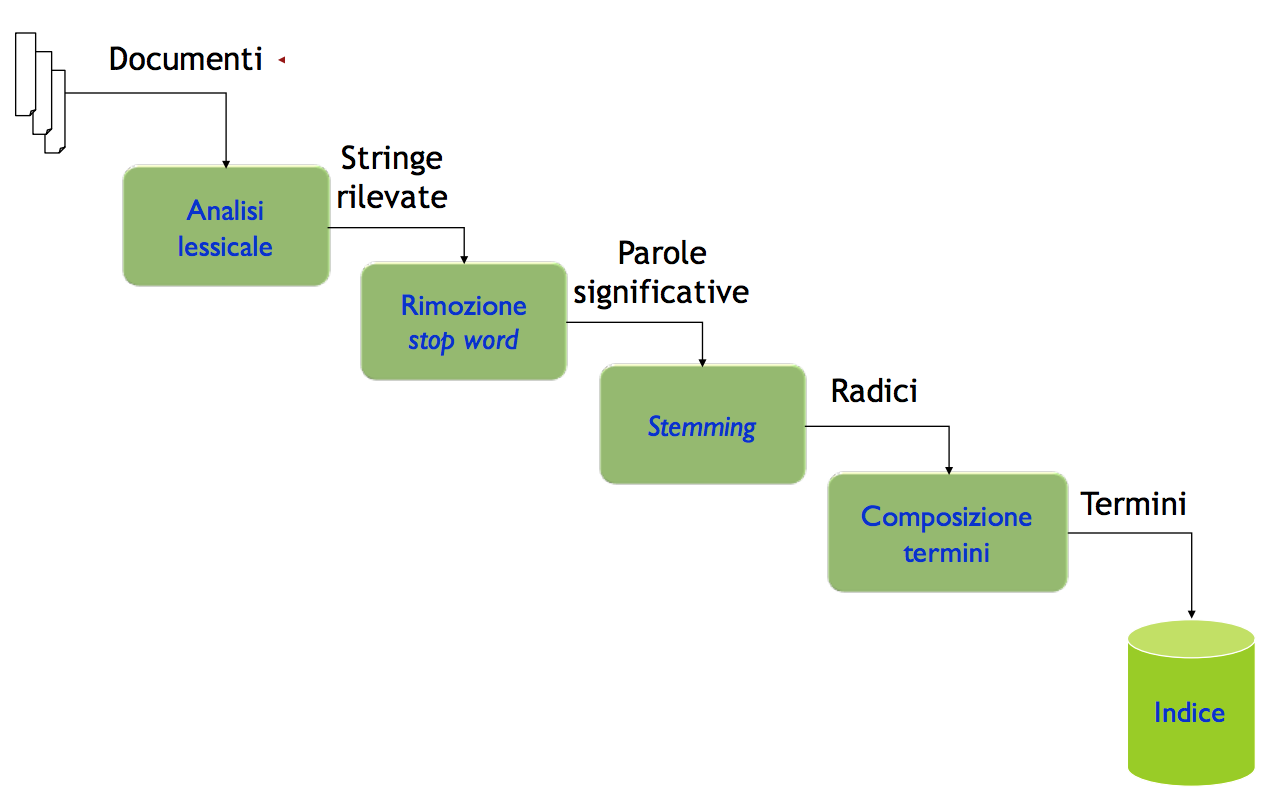
\includegraphics[width=0.7\linewidth]{images/l12-fig-3.png}
\end{figure}

\noindent Le varie proprietà del file properties influiscono sulla fase di analisi lessicale nel seguente modo:

\begin{itemize}
	\item \textbf{Documenti}: specificati nel file \texttt{collection.spec}
	\item \textbf{Analisi lessicale}:
	\begin{itemize}
		\item \texttt{tokeniser=EnglishTokenize}: che tokenizer utilizzare, dipende dalla lingua dei documenti.
		\item \texttt{trec.encoding=UTF-8}: codifica dei caratteri, noi utilizziamo UTF-8 perché dobbiamo gestire anche le lettere accentate e i caratteri in cirillico. Utilizzare UTF-16 è un over-kill, può essere utile con le lingue giapponesi.
		\item \texttt{trec.collecion.class=SimpleFileCollection} e \texttt{trec.document.class=FileDocument}: specificano le classi Java da utilizzare per fare la tokenizzazione (analisi lessicale). In questo caso \texttt{SimpleFileDocument} permette di indicizzare file di testo, mentre per utilizzare documenti strutturati serve un'altra classe.
	\end{itemize}
	\item \textbf{Rimozione stop-word}:
	\begin{itemize}
		\item \texttt{stopwords.filename=stopword.txt}: file con le stop-word.
		\item \texttt{termpipelines=Stopwords}: aggiunge nella pipeline la rimozione delle stop-word.
	\end{itemize}
	\item \textbf{Stemming}: \texttt{termpipelines=PorterStemmer} per la selezione dello stemmer da utilizzare.
	\item \textbf{Composizione termini}: niente.
	\item \textbf{Indice}:
	\begin{itemize}
		\item \texttt{index.meta.forward.keys=filename}: codice per riferirsi ai documenti indicizzati. Con questa impostazione viene utilizzato il nome del file.
		\item \texttt{index.meta.forward.keylens=512}: dimensione della chiave.
	\end{itemize}
\end{itemize}

\noindent Per avviare l'indicizzazione viene utilizzato lo script:

\begin{centering}
	\texttt{\$ sh bin/trec\_terrier.sh -i}
\end{centering}


\noindent L'indice così prodotto viene messo nella cartella \texttt{var/index}, ma può essere modificata dal file properties.

Al comando di creazione dell'indice è possibile passare dei flag per fargli stampare un po' di informazioni:

\begin{itemize}
	\item \texttt{--printlexicon} contenuto del ``lexicon''
	\item \texttt{--printinverted} contenuto dell'``inverted file''
	\item \texttt{--printdirect} contenuto del ``direct file''
	\item \texttt{--printstats} statistiche
	\item \texttt{--printmeta} the meta structure
\end{itemize}

\noindent Una possibile riga del lexion prodotto è

\begin{center}
	\textit{direct,term55 Nt=5 TF=8 \@{0 122 2}}
\end{center}

\noindent La prima cosa è il termine stemmato, il secondo è l'identificatore progressivo, c'è poi il numero di documenti contenti il termine (\textit{Nt}) e la term frequency (\textit{TF}) nella collezione. L'ultima parte è un'informazione interna di Terrier.

Nell'indice trasposto le informazioni sono memorizzate con un'identificativo interno del documento.
Una riga dell'indice trasposto è:

\begin{center}
	\textit{513 (0,2) (1,1) (3,2)}
\end{center}

\noindent Dove il primo campo è l'identificativo del termine, mentre le coppie contengono l'identificativo del documento e la \textit{TF} del termine all'interno del documento.
Da notare che il l'identificativo del termine (\textit{es: 513}) non viene inserito all'interno del lexicon, è necessario fare affidamento al numero di rigua.

\section{Indicizzazione e interrogazione di documenti non in inglese}

La collezione di riferimento è adesso in italiano ed in formato pdf. Può essere recuperata all'url \texttt{www.dei.unipd.it/~silvello/IR2016-2017/small\_test\_collections/pdf/}.

Le modifiche da fare riguardano:

\begin{itemize}
	\item \texttt{tokeniser=UTFTokeniser}: perché ci sono gli accenti. Stranamente utilizzare questo tokeniser con l'inglese da dei problemi.
	\item \texttt{trec.document.class=PDFDocument}: perché stiamo utilizzando dei pdf.
	\item \texttt{stopwords.filename=.../italian\_stoplist.txt}: perché servono le stop-words specifiche per la lingua.
	\item \texttt{termpipelines=ItalianSnowballStemmer}: un altro stemmer interno di Terrier creato per la lingua italiana. Nel nostro progetto abbiamo uno stemmer statistico e quindi non dovremmo andare a cambiare questo parametro quando cambiamo lingua.
\end{itemize}

\section{Configurazione di Terrier per il nostro progetto}

Una volta creato lo stemmer statistico, per farlo utilizzare a Terrier dobbiamo specificare le seguenti proprietà:

\begin{lstlisting}
termpipeline=LookupStemmer
lookupstemmer.filename=<pathToFile> // verso il file prodotto dal nostro script
lookupstemmer.encoding=UTF-8
tokenizer=UTFTokenizer
\end{lstlisting}

\noindent Per generare il dizionario completo delle parole non dobbiamo specificare lo stemmer.

Per il progetto non è richiesto l'uso di stop-list, ma se si voglio fare dei test extra è possibile utilizzarle.



